\documentclass[twoside]{article}

\usepackage[math]{kurier}
\usepackage[sc]{mathpazo}
\usepackage{graphicx}
\usepackage{caption}
\usepackage{subcaption}
\usepackage{url}
\usepackage[]{algorithm2e}
\usepackage{amstext,amsmath,amssymb,epsfig,fancyhdr}
\renewcommand{\sfdefault}{kurier}

\setlength{\oddsidemargin}{0.25 in}
\setlength{\evensidemargin}{-0.25 in}
\setlength{\topmargin}{-0.6 in}
\setlength{\textwidth}{6.5 in}
\setlength{\textheight}{8.5 in}
\setlength{\headsep}{0.75 in}
\setlength{\parindent}{0 in}
\setlength{\parskip}{0.1 in}


\newcounter{lecnum}
\renewcommand{\thepage}{\thelecnum-\arabic{page}}
\renewcommand{\thesection}{\thelecnum.\arabic{section}}
\renewcommand{\theequation}{\thelecnum.\arabic{equation}}
\renewcommand{\thefigure}{\thelecnum.\arabic{figure}}
\renewcommand{\thetable}{\thelecnum.\arabic{table}}


\newcommand{\lecture}[4]{
   \pagestyle{myheadings}
   \thispagestyle{plain}
   \newpage
   \setcounter{lecnum}{#1}
   \setcounter{page}{1}
   \noindent
   \begin{center}
   \framebox{
      \vbox{\vspace{2mm}
    \hbox to 6.28in { {\bf \sffamily AA 274: Principles of Robotic Autonomy
                        \hfill Winter 2019} }
       \vspace{4mm}
       \hbox to 6.28in { {\sffamily{\Large \hfill Lecture #1: #2  \hfill}} }
       \vspace{2mm}
       \hbox to 6.28in { {\it \hfill Scribes: #4} }
      \vspace{2mm}}
   }
   \end{center}
   \markboth{Lecture #1: #2}{Lecture #1: #2}

   \vspace*{4mm}
}



%%%%%%%%%%%%%%%%%%%%%%%%%%
%document
\begin{document}
%modify this
\lecture{10}{Object Localization and Detection}{}{}

\section{Introduction}

We finished covering the material for Homework 2 and we are moving on to the third topic of this class, which is localization.  The goal of localization is to use information gathered from the sensing and perception modules in order to determine where the robot is with respect to the world.

Localization incorporates the use of probabilistic methods, as there will always be uncertainty in a robot's position.  Therefore, lecture 10 will cover an introduction to probability, including belief representation and Bayes' rule. We will use these topics to introduce the Bayes' filtering algorithm, a theoretically sound but potentially impractical algorithm that uses the state transition model and sensor measurements to generate the belief state.
 
% lecture 10
\section{Localization}
\subsection{Behavioral Approach}

\begin{figure}[h!]
	\centering
    \includegraphics[width=0.6\textwidth]{img/Siegwart_5_6.png}
    \caption{Siegwart Figure 5.6. An environment with rooms A and B}
    \label{fig:siegwart_5_6}
\end{figure}

Behavioral approach attempts to design a set of behaviors that result in desired robot motion and trajectory. This method avoids mapping the robot's environment for localization. For example, consider Fig.~\ref{fig:siegwart_5_6}, where a robot wants to navigate from room A to room B. Using behavioral approach, a robot may find its way to room B by following the left wall, incorporating other procedures such as collision avoidance and identification of room B. However, compared to map-based approach, this method of navigation has difficulty scaling to different problems or environments. Depending on situations, techniques like following the left wall can also be suboptimal.

\subsection{Map-based Approach}

Map-based localization uses information about the robot's surrounding to identify its position \textit{with respect to} the environment. To gain knowledge of its environment, the robot must actively gather and process sensor data of the surrounding. The most popular sensor is LIDAR, which can provide $360^\circ$ coverage of the robot's surrounding. This approach can scale to any kind of environment, because a robot can use same techniques and sensors to map its surrounding.

\begin{figure}[h!]
	\centering
    \includegraphics[width=0.8\textwidth]{img/Siegwart_maps.png}
    \caption{Siegwart Figure 5.10. (a) Real map. (b) Map where continuous lines represent walls. (c) Same map discretized into 3000 grid cells. (d) Topological map with nodes and edges.}
    \label{fig:siegwart_maps}
\end{figure}

\subsection{Belief representation}
Due to sensor noise, a robot cannot localize itself with absolute certainty. To compensate for the error, we can represent the estimate of robot's location as a probability distribution across the environment. There are different ways of representation. For example, the belief of robot's position can be \emph{continuous}, which can be expressed by continuous variables $(x, y, \theta)$ Fig.~\ref{fig:siegwart_maps}(b). \\

On the other hand, the belief can be \emph{discrete}. For instance, the map of the environment may be discretized into $N \times N$ cells as in Fig.~\ref{fig:siegwart_maps}(c), and the belief can assign probabilities of being in different cells. The other possible discrete representation is a topological map in Fig.~\ref{fig:siegwart_maps}(d), which maps the environment using nodes and edges. We can then assign probabilities of robot being in certain nodes. \\

\begin{figure}[h!]
	\centering
    \includegraphics[width=0.8\textwidth]{img/Siegwart_beliefs.png}
    \caption{Siegwart Figure 5.9. (a) Continuous single-hypothesis belief. (b) Continuous multiple-hypothesis belief. (c) Discrete probabilities for grid-based map. (d) Discrete probabilities for topological map.}
    \label{fig:siegwart_beliefs}
\end{figure}

The belief representation can also be classified as either \emph{single-hypothesis belief} or \emph{multiple-hypothesis belief}. \emph{Single-hypothesis belief}, as in Fig.~\ref{fig:siegwart_beliefs}(a), is useful when describing a unique estimate of a robot's position. On the other hand, \emph{multiple-hypothesis belief} in Fig.~\ref{fig:siegwart_beliefs}(b, c, d) can be used to describe multiple possible locations of a robot. \\

Continuous belief representation typically incorporates single-hypothesis belief (ex. state vector [$x, y, \theta$]) that is compact and easy to compute. However, discrete belief representation typically incorporates multiple-hypothesis belief. Because discrete method assigns the probabilities of robot's presence across different cells or nodes in the map, we see that the accuracy of estimate is limited by the resolution of discretization. It may also involve heavy computation, because a robot must keep track of probabilities associated each cell \cite{Clark}.

\section{Probability Basics}

\subsection{Random Variable}

Quantities such as sensor measurements, states of a robot and its environment are modeled as random variables. A random variable is a variable whose possible values are outcomes of a random phenomenon. In the case of sensor measurements, the source of randomness could be sensor noise. Random variables fall under one of two categories: discrete or continuous.

\subsubsection{Discrete Random Variable}

Discrete random variables can take on only a countable number of values. For example, if we flip a coin twice and the random variable $X$ represents the number of coin flips resulting in "heads", $X$ can only take on values of 0, 1 or 2 (and similarly for the case of "tails"). A discrete random variable is characterized by a probability mass function (PMF) $p(X=x)$ (or $p(x)$) where
\begin{center}
$\sum\limits_{x} p(x)=1$.
\end{center}

\subsubsection{Continuous Random Variable}

In contrast with a discrete random variable, a continuous random variable can take on an infinite number of values. A continuous random variable is characterized by a probability density function (PDF), $p(x)$, where the probability of a random variable being contained within the interval $[a,b]$ is
\begin{center}
$P(a \leq X \leq b) = \int_{a}^{b}p(x)dx$
\end{center}
where
\begin{center}
$\int_{-\infty}^{+\infty}p(x)dx=1$.
\end{center}

\subsection{Joint Distributions, Independence and Conditional Probability}

\subsubsection{Joint Distributions}

The joint distribution of two random variables $X$ and $Y$ is denoted as \begin{center}
$p(x,y):=p(X=x\ \textnormal{and}\ Y=y).$
\end{center}

\subsubsection{Independence}

If $X$ and $Y$ are random variables such that,
\begin{center}
$p(x,y)=p(x)p(y)$
\end{center}
then $X$ and $Y$ are said to be independent.

\subsubsection{Conditional Probability}

Conditional probability is the probability of an event happening given that another event has occurred. That is, suppose that we know that the event $Y = y$ occurs with probability $p(y) > 0$. The probability of the event $X=x$ occurring given that $Y=y$ has occurred, or alternatively stated as the conditional probability of $X$ given $Y$, is given by

\begin{center}
$p(x|y):=\frac{p(x,y)}{p(y)}.$
\end{center}

Thus if $X$ and $Y$ are independent, $p(x|y)=p(x)$. Also, note that the above definition of conditional probability is indeed a definition and not theoretically derived.

In order to better understand the concept of conditional probability, consider Fig. ~\ref{fig:cond_prob_example}\. In this figure, the sample space $\Omega$ contain the set of all possible outcomes for a random variable. Consider the case where there are two possible outcomes, $B1$ and $B2$ which may occur with an equal probability of $0.5$. These events correspond to the orange and blue regions of $\Omega$, respectively. An event $A$ that occurs with probability $0.5$ can also be defined, which corresponds to the centered shaded region in Fig. ~\ref{fig:cond_prob_example}.

Suppose that we wish to determine the probability of $A$ occurring and that a sample from $\Omega$ is observed to result in the event $B1$. Given that $B1$ has occurred, we restrict our attention to the region $B1$. In this restricted region, the area corresponding to $A$ occurring is the intersection of $A$ and $B1$. Since region $A$ overlaps with half of the region $B1$, we have the result that $p(A|B1) = 0.5.$ A slightly different but equivalent interpretation of this figure, as given during lecture, is that we rescale the probability of event $A$ occurring by the probability of the event that has happened. Mathematically, this is expressed as

\begin{center}
$p(A|B1)=\frac{p(A \cap B1)}{p(B1)}=\frac{0.25}{0.5}=0.5.$
\end{center}

\begin{figure}[h!]
	\centering
    \includegraphics[width=0.6\textwidth]{img/Cond_Prob_Example.png}
    \caption{Sample space representation. Note that region A is centered an overlaps $B1$ and $B2$ equally.}
    \label{fig:cond_prob_example}
\end{figure}

Finally, note that if $X$ and $Y$ are independent $p(x|y):=p(x)$.
\subsubsection{Conditional Independence}
If $X$, $Y$ and $Z$ are random variables such that,
\begin{center}
$p(x,y \mid z)=p(x \mid z)p(y \mid z)$
\end{center}
then $X$ and $Y$ are said to be conditionally independent given $Z$. \newline
However:
\begin{center}
$p(x,y \mid z)=p(x \mid z)p(y \mid z) \not \Rightarrow p(x,y)=p(x)p(y)$
\end{center}
Nor:
\begin{center}
$p(x,y)=p(x)p(y) \not \Rightarrow p(x,y \mid z)=p(x \mid z)p(y \mid z)$
\end{center}
\subsection{Theorem of Total Probability}

Once again consider Fig. ~\ref{fig:cond_prob_example}. If we wished to find the probability of $A$ without any assumptions regarding conditioning, we can do so by calculating

\begin{center}
$p(A)=p(A \cap B1) + p(A \cap B2).$
\end{center}

This idea can be generalized for discrete random variables into what is known as the theorem (or law) of total probability as

\begin{center}
$p(x)=\sum\limits_{y}p(x,y)=\sum\limits_{y}p(x|y)p(y)$
\end{center}

where the definition of conditional probability was used to obtain the last expression. For continuous random variables, the summations simply turn into integrals:

\begin{center}
$p(x)=\int p(x,y)dy=\int p(x|y)p(y)dy$
\end{center}

\subsection{Bayes' Rule}

To facilitate the explanation of Bayes' Rule please note: a sample space is a set containing all the possible outcomes of an experiment and an event is a subset of elements in a sample space. Imagine that there is an event $A$ whose set of outcomes is contained in the sets of events $B_i$ where $i = 0, 1, ..., n$ of a sample space. For example in Fig. ~\ref{fig:cond_prob_example}\ event A's set is contained in the sets of events $B_1$ and $B_2$. Then,

\begin{center}
$p(B_i|A)=\frac{p(B_i \cap A)}{p(A)}$.
\end{center}

Using the formula for conditional probability $p(B_i \cap A)$ and $p(A)$ can be expressed as:

\begin{center}
$p(B_i \cap A)= p(A|B_i)p(B_i) $.

$p(A)= \sum\limits_{i = 0}^{n} p(B_i \cap A) = \sum\limits_{i = 0}^{n} p(A|B_i)p(B_i)$.
\end{center}

Combining these two expressions to derive Bayes' Rule for discrete sample spaces:

\begin{center}
$p(B_i|A)= \frac{p(A|B_i)p(B_i)}{\sum\limits_{i = 0}^{n} p(A|B_i)p(B_i)}$.
\end{center}

For a continuous sample space Bayes' Rule is:

\begin{center}
$p(B|A)= \frac{p(A|B)p(B)}{\int p(A|B = b')p(B = b')db'}$.
\end{center}

Note that $p(A)$ is independent of which event $Bi$ is selected. So the denominator of Bayes' formula can be considered a constant for all events $Bi$ with event $A$. Furthermore, by knowing the probabilities $p(A|Bi)$ and $p(Bi)$, we can determine $p(Bi|A)$. As an example, a brewery buys equal amounts of hops from two farmers, $B1$ and $B2$. The brewery has a strict policy of using only one type of hops in each batch of beer it brews. Furthermore, the brewery uses half of all its hops from both sources to produce Pilsner beer. Bayes' Rule can be applied to determine, given that a batch of Pilsner is produced, what is the probability that the batch was brewed using hops from farmer $B1$. Note this example uses the sample space described in Fig. ~\ref{fig:cond_prob_example}\

\begin{center}
$p(B_1|A)= \frac{p(A|B_1)p(B_1)}{\sum\limits_{i = 0}^{1} p(A|B_i)p(B_i)} = \frac{p(A|B_1)p(B_1)}{p(A|B_1)p(B_1) + p(A|B_2)p(B_2)} = \frac{0.5*0.5}{(0.5*0.5 + 0.5*0.5)} = \frac{0.25}{0.5} = 0.5$.
\end{center}

Bayes' Rule can be extended with the use of additional random variables. In the three variable case, given $X=x$, $Y=y$ Bayes' Rule can be conditioned on an additional variable $Z=z$ as follows:

\begin{center}
$p(x|y, z)= \frac{p(y|x,z)p(x|z)}{p(y|z)}$.
\end{center}

This is the probability that event $Z=z$, and event $X=x|Y=y$ occur, which describes $Z=z$ influence on joint event $X=x|Y=y$.

\subsection{Expectation and Covariance}

The expectation value of a random variable $E(X)$ is the average result of an experiment over an infinite number of trials. It is also known as the first moment of the distribution. For the discrete case:

\begin{center}
$E(X)= \sum\limits_{i = 0}^{n} x_ip(X=x_i)$.
\end{center}

For the continuous case:

\begin{center}
$E(X)= \int\limits_{-\infty}^{\infty}  x'p(X=x')dx'$.
\end{center}

The expectation value of a constant is a constant and its calculation is a linear operation.

\begin{center}
$E(aX + b)= aE(X) + b$.
\end{center}

In the case of a vector of random variables. The expectation of the vector is the vector of each variables expectation value.

Covariance is a calculation used to measure the relationship between random variables. For two random variable vectors $X=x, Y=y$, the covariance is:

\begin{center}
$cov(X,Y)=E[(X-E(X))(Y-E(Y))] = E(XY^T) - E(X)E(Y^T)$
\end{center}

If the covariance is positive this implies that X tends to increase at the same time as Y. If the covariance is negative then this implies that X tends to decrease as Y increases.If changes in X and Y have a random relationship, then the covariance will be close to zero. If two variables have a covariance of zero they are called uncorrelated. If two variables are independent they will be uncorrelated. However, two variables which are uncorrelated are not always independent.

\section{Model for robot-environment interaction\cite{thrun2005probabilistic}}
There are two fundamental types of robot-environment interaction:
\begin{enumerate}
  \item The robot can acquire information about its environment using its sensors.

  \item The robot can also influence its environment through its actuators.
\end{enumerate}
\subsection{State}
We define the state($x$) as the collection of all aspects
of the robot and its environment that can impact the future.$x_{t}$ denote the state at time t. In addition, we define notation: $x_{t_1:t_2} := x_{t_1},x_{t_1+1},...,x_{t_2}$. 
State variables include:
\begin{itemize}
  \item Robot	pose	(e.g.,	robot	location	and	orientation relative to a
global coordinate frame)
  \item Robot	velocity
  \item Location	and	features	of	surrounding	objects	in	the	environment,	etc
\end{itemize}

A state $x_{t}$ will be called complete if it is the best predictor of the future. The future may be stochastic, but no variables prior to $x_{t}$ may influence the stochastic evolution of future states, unless this dependence is mediated through the state $x_{t}$. Temporal processes that meet these conditions are only known as Markov chains(Markov property).

\subsection{Measurement and control data}
Environment measurement data provides information about a momentary state of the environment. The measurement data at time $t$ will be denoted $z_{t}$.We define notation: $z_{t_1:t_2} := z_{t_1},z_{t_1+1},...,z_{t_2}$, denotes the set of all measurements acquired from time $t_1$ to time $t_2$, for
$t_1 \leq t_2$.\par

Control data carry information about the change of state in the environment.In mobile robotics, a typical example of control data is the velocity
of a robot.Control data will be denoted $u_t$. The variable $u_t$ will always correspond to
the change of state in the time interval (t-1;t].We define notation: $u_{t_1:t_2} := u_{t_1},u_{t_1+1},...,u_{t_2}$, denotes the sequences of control data from time $t_1$ to time $t_2$, for
$t_1 \leq t_2$.\par

 Environment perception provides information about the environment’s state, hence it tends to increase the robot’s knowledge. Motion, on  the other hand, tends to induce a loss of knowledge due to the inherent noise in robot actuation and the stochasticity of robot environments.
 
 \subsection{State equation}
 The evolution of state and measurements is governed by probabilistic laws. the probabilistic law characterizing
the evolution of state might be given by a probability distribution
of the following form: $p(x_t \mid x_{1:t-1}, z_{1:t-1}, u_{1:t})$. Notice that through no particular
motivation we assume here that the robot executes a control action $u_1$ first, and then takes a measurement $z_1$.

 If the state x is complete then it is a
sufficient summary of all that happened in previous time steps. In particular,$x_{t-1}$ is a sufficient statistic of all previous controls and measurements up to this point in time, that is, $u_{1:t-1}$ and $z_{1:t-1}$. From all the variables in the
expression above, only the control $u_t$ matters if we know the state $x_{t-1}$. That is :

\begin{center}
$p(x_t \mid x_{1:t-1}, z_{1:t-1}, u_{1:t}) = p(x_t \mid x_{t-1},u_t)$
\end{center}

\subsection{Measurement equation}
The probability of getting a measurement $z_t$ is also given by a probabilistic law. Again, if we assume that the state $x$ is complete, then we can say that state $x_t$ already encodes the effect of all previous states $x_{0:t-1}$, previous measurements, $z_{1:t-1}$, and previous controls $u_{1:t}$. This allows us to arrive at the equation:  

\begin{center}
$p(z_t \mid x_{0:t},z_{1:t-1},u_{1:t})=p(z_t\mid x_t)$
\end{center}

\subsection{Overall stochastic model}
It is important to keep the order of occurrence of different events in the model consistent. In our notation, we assume that the control effort $u_t$ is determined after taking into account the state $x_{t-1}$ and measurement $z_{t-1}$. The control effort $u_t$ causes the robot to transition to a new state $x_t$ where a new measurement $z_t$ is taken, which in turns allows the determination of a new control effort $u_{t+1}$. This network model is a stochastic model known as a Markov process because the new state $x_t$ only depends on the previous state $x_{t-1}$ and the previous control $u_t$. In addition, since we cannot directly observe the current state, but instead estimate it through measurements, this model is further classified as a hidden Markov model. 

\begin{figure}[h!]
	\centering
    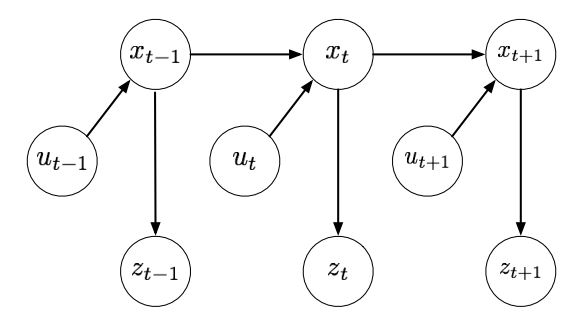
\includegraphics[width=0.6\textwidth]{img/HMV.jpg}
    \caption{Overall	dynamic	Bayes	
network	model (Hidden Markov Model)}
    \label{fig:cond_prob_example}
\end{figure}

\subsection{Belief distribution}
We can encode our internal knowledge of the state in a belief distribution, which is a probability distribution that has a value for each possible hypothesis of the true state. Formally, our belief distribution at a particular state is the probability of being at that state given all the measurements and control efforts we've seen so far. 

\begin{center}
$bel(x_t):=p(x_t\mid z_{1:t},u_{1:t})$
\end{center} 

Note that this probability distribution can be unimodal or multimodal. A useful tool to calculate our belief distribution is an intermediate belief distribution known as the prediction distribution. The prediction distribution is the probability of being at a state given all the past measurements (except the one we took at this new state) and the previous control efforts. 

\begin{center}
$\overline{bel}(x_t):=p(x_t\mid z_{1:t-1},u_{1:t})$
\end{center} 

Therefore, the first step to calculate our final belief distribution is to calculate the prediction distribution. Next, we add the latest measurement to sharpen the belief. This second step of calculating the true belief from the prediction belief is called the correction step or the measurement update.  This leads us to the Bayes filter algorithm. 

\section{Bayes' filter algorithm}
The Bayes' filter algorithm is the most general algorithm for calculating state beliefs. The key assumption made in this algorithm is that the state $x_t$ is complete, i.e. only depends on the previous state and control effort, $x_{t-1}$ and $u_t$. Note that the Bayes' filter algorithm is the most general algorithm but is not necessarily achievable. The algorithm assumes a continuous state space, continuous time, and requires that we be able to compute all the beliefs in an arbitrarily dimensionally large space. Though not practical, the Bayes' filter algorithm is still a great starting point to derive more practical algorithms that can be used in different scenarios. 

\subsection{Overview of algorithm}
This is a recursive algorithm. It is initialized with some guess of the initial state, i.e. an initial belief $bel(x_0)$. This can be a uniform distribution of density or point masses if we have no prior information. \\
The first step is to carry out the prediction step to compute $\overline{bel}(x_t)$ using the previous control effort $u_t$ used to get to state $x_t$. This is simply the integration over all possible previous states $x_{t-1}$, of the product of the prior belief $bel{x_{t-1}}$ (where we think we were before) and the transition model given that we know our last control effort $p(x_t \mid u_t, x_{t-1})$. This prediction belief is an encoding of how likely it is that we're now at $x_t$.
\begin{center}
$\overline{bel}(x_t)= \int p(x_t \mid u_t, x_{t-1}) bel({x_{t-1}}) dx_{t-1}$
\end{center}
The second step is the measurement update where the most recent measurement is incorporated to sharpen our belief. This involves taking our prediction belief and multiplying it by the probability of seeing the measurement that we did $z_t$ if we were actually at our predicted state $x_t$. This allows us to correct our prediction belief and find our true belief. 
\begin{center}
$bel(x_t):=\eta p(z_t\mid x_t) \overline{bel}(x_t) $
\end{center} 
After these two steps, a control effort $u_{t+1}$ is taken, we transition to a new state $x_{t+1}$, and the process of prediction and measurement update is repeated. This is what makes the Bayes' filter algorithm a recursive algorithm. 

\subsection{Derivations}
The second step of the Bayes' Filter Algorithm involves the measurement update of our belief model. Here we will go into further detail regarding the derivation of the measurement update.

We begin with our belief
\begin{equation*}
    bel(x_{t}) = p(x_{t}|z_{1:t},u_{1:t})
\end{equation*}
We then expand this using Bayes' Rule to get:
\begin{equation*}
    bel(x_{t}) =\frac{p(z_{t}|x_{t}z_{1:t-1},u_{1:t})p(x_{t}|z_{1:t-1},u_{1:t})}{p(z_{t}|z_{1:t-1},u_{1:t})} 
\end{equation*}
Where the denominator is the normalizor and is equal to $\eta^{-1}$. Next, we use the Markov Property to get:
\begin{equation*}
    bel(x_{t}) = \eta p(z_{t}|x_{t})p(x_{t}|z_{1:t-1},u_{1:t})
\end{equation*}
Where the right term equates to the prediction distribution $\overline{bel}(x_{t})$.
Next we derive the Correction Update that we perform on that prediction distribution
\begin{equation*}
    \overline{bel}(x_{t}) = p(x_{t}|z_{1:t-1},u_{1:t})
\end{equation*}
Using the law of total probability, we expand to get:
\begin{equation*}
    \overline{bel}(x_{t}) = \int p(x_{t}|x_{t-1},z_{1:t-1},u_{1:t})p(x_{t-1}|z_{1:t-1},u_{1:t})dx_{t-1}
\end{equation*}
Next we use the Markov Property to simplify the left term:
\begin{equation*}
    \overline{bel}(x_{t}) = \int p(x_{t}|x_{t-1},u_{t})p(x_{t-1}|z_{1:t-1},u_{1:t})dx_{t-1}
\end{equation*}
For general output feedback policies, $u_{t}$ does not provide feedback additional information on $x_{t-1}$ and so:
\begin{equation*}
    \overline{bel}(x_{t}) = \int p(x_{t}|x_{t-1},u_{t})p(x_{t-1}|z_{1:t-1},u_{1:t-1})dx_{t-1}
\end{equation*}
The right term then simplifies so that we get our result:
\begin{equation*}
    \overline{bel}(x_{t}) = \int p(x_{t}|x_{t-1},u_{t})bel(x_{t-1})dx_{t-1}
\end{equation*}
\subsection{Discrete Bayes' filter algorithm}

For problems with finite state spaces, a Discrete Bayes' Filter can be implemented. Initially, we represent the belief state, $bel(x_{t})$, as a probability mass function $\{p_{k,t}\}$. The pseudo code for the algorithm is shown below:
\\
\\
\begin{algorithm}[H]
 \KwData{$\{p_{k,t-1}\}, u_{t},z_{t}$}
 \KwResult{$\{p_{k,t}\}$}
 initialization\;
 \ForEach{k}{
  $\overline{p}_{k,t}=\Sigma_{i} p(X_{t} = x_{t}|u_{t},X_{t-1}=x_{i})p_{i,t-1} $\;
  $p_{k,t}=\eta p(z_{t}|X_{t} = x_{k})\overline{p}_{k,t}$\;
 }
 \Return $p_{k,t}$
 \caption{Discrete Bayes' Filter Algorithm}
\end{algorithm}

\section{Additional Resources}

There are some additional resources to which you can refer. Chapter 2 in \cite{thrun2005probabilistic} provided basic probabilistic concepts that are frequently used in robotics, the formal model of robot interaction, introduction to \textit{Bayes filters} and implementing issues associated with that. 

If you want to dive deeper into \textit{Bayes filters}, \cite{sarkka2013bayesian} is a comprehensive book on Bayesian filtering and smoothing and applications of \textit{Bayes filters} such as \textit{Kalman filters} (including extended and unscented \textit{Kalman filters}), \textit{Gaussian filters} and \textit{Particle filters}. As you know, Bayes recursive filter is not a practical algorithm, which means it cannot be implemented on a computer. Therefore, it is important to understand those implementations using the principle of \textit{Bayes filters}. 

If you are interested in the original paper on \textit{Kalman filters} by R.E.Kalman, you can refer to \cite{kalman1960new}. This famous paper described a recursive solution to discrete filtering problem. With the advance of computer and robotics, this paper inspired a lot of researches and applications. 

There is a great online article \cite{HowKF} which provides an intuitive explanation of what is a \textit{Kalman filters} and how it works. This article approaches \textit{Kalman filters} in a slightly different way (more from a linear algebra point of view). Nevertheless, it will help you build insightful intuitions of \textit{Kalman filters} and is very interesting to read through.


\bibliographystyle{ieee}
\bibliography{egbib}

\subsubsection*{Contributors}
Winter 2019: Akshay Gupta, Ian Vorbach, Orien Zeng, Somrita Banerjee, Zhengyu Chen
\\
Winter 2018: Junjie Ke, Ryan Wong, Amine Elhafsi, Samuel Sowell, Peter Zachares
\end{document}
